\documentclass[handout]{beamer}

\usepackage[T2A]{fontenc}
\usepackage[utf8]{inputenc}
\usepackage[russian]{babel}
\usepackage{graphicx}
\usepackage{todonotes}
\usepackage{listings}
\usepackage{adjustbox}

\usetheme{Madrid}
\usecolortheme{whale}

\hypersetup {
    unicode = true
}

\lstset{
  extendedchars={true},
  inputencoding={utf8},
  language={Java},
  basicstyle={\ttfamily \scriptsize},
  keywordstyle={\rmfamily \bfseries},
  commentstyle={\rmfamily \itshape},
  tabsize={2},
  frame={single},
  showstringspaces={false},
  breaklines={true},
}

\title[Инструментальная среда]{Инструментальная среда для анализа программных систем}
\author[А.М. Половцев]{
    А.М. Половцев, гр. 63501/13\\
    научный руководитель: к.т.н. доцент В.М. Ицыксон\\[3ex]
    Направление: 230100 -- Информатика и вычислительная техника\\
    Магистерская программа: 230100.68.15 –- Технологии проектирования
системного и прикладного программного обеспечения
}
\institute[СПбГПУ]{Санкт-Петербургский государственный политехнический университет}
\date[10 июня 2014~г.]{10 июня 2014~г.}

\begin{document}
%===============================================================================
\frame{\titlepage}
%===============================================================================
%===============================================================================
\begin{frame}
\frametitle{Актуальность}

\begin{itemize}
    \item Растет сложность и размер программных систем
    \item Снижаются сроки разработки
    \item Эти факторы ведут к падению уровня качества
    \item В различных методах повышения качества часто решаются похожие задачи:
    \begin{itemize}
        \item Построение моделей программы (AST, CFG, \ldots)
        \item Построение метрик
        \item Реинжиниринг программного обеспечения (оптимизация, рефакторинг, \ldots)
        \item Визуализация свойств системы
    \end{itemize}
\end{itemize}

\begin{alertblock}{}
    \center{Обычно эти задачи решаются вручную для каждого языка программирования}
\end{alertblock}

\end{frame}
%===============================================================================
%===============================================================================
\begin{frame}
\frametitle{Рассматриваемый подход}

\begin{itemize}
    \item Решение данной проблемы основывается на использовании промежуточного
    представления, не зависящего от языка программирования, на котором написана
    анализируемая система
    \item \textbf{Метамодель} - модель, описывающая язык для формулировки моделей
    \item Поиск компромисса между степенью детализации и уровнем абстракции
\end{itemize}

\end{frame}
%===============================================================================
%===============================================================================
\begin{frame}
\frametitle{Решаемые задачи}

\begin{itemize}
    \item В итоге требуется решить следующие задачи:
        \begin{itemize}
            \item Проектирование промежуточного представления, не зависящего от
            языка программирования анализируемой системы, для применения
            обобщенных процедур анализа
            \item Разработка графической инструментальной среды на основе
            промежуточного представления для визуализации моделей, метрик и
            свойств программных систем с целью повышения уровня качества
        \end{itemize}

\end{itemize}

\end{frame}
%===============================================================================
%===============================================================================
\begin{frame}
\frametitle{Требования}

\begin{itemize}
    \item Требования к промежуточному представлению
        \begin{itemize}
            \item Независимость от языка описания анализируемой системы
            \item Расширяемость
            \item Простота в использовании
            \item Полнота
        \end{itemize}
    \item Требования к инструментальной среде
        \begin{itemize}
            \item Визуализация извлеченных моделей
            \item Подсчет метрик
            \item Визуализация дополнительных свойств
        \end{itemize}
\end{itemize}

\end{frame}
%===============================================================================
%===============================================================================
\begin{frame}
\frametitle{Существующие решения}

\begin{itemize}
    \item Moose - слишком громоздкая метамодель
    \item LLVM - низкоуровневое промежуточное представление
    \item SMIILE - ориентирован только на метрики
    \item Ulf-Ware - представление только для языков Java и C++
\end{itemize}

\end{frame}
%===============================================================================
%===============================================================================
\begin{frame}
\frametitle{Архитектура программной системы}

\begin{figure}[b!]
    \begin{center}
        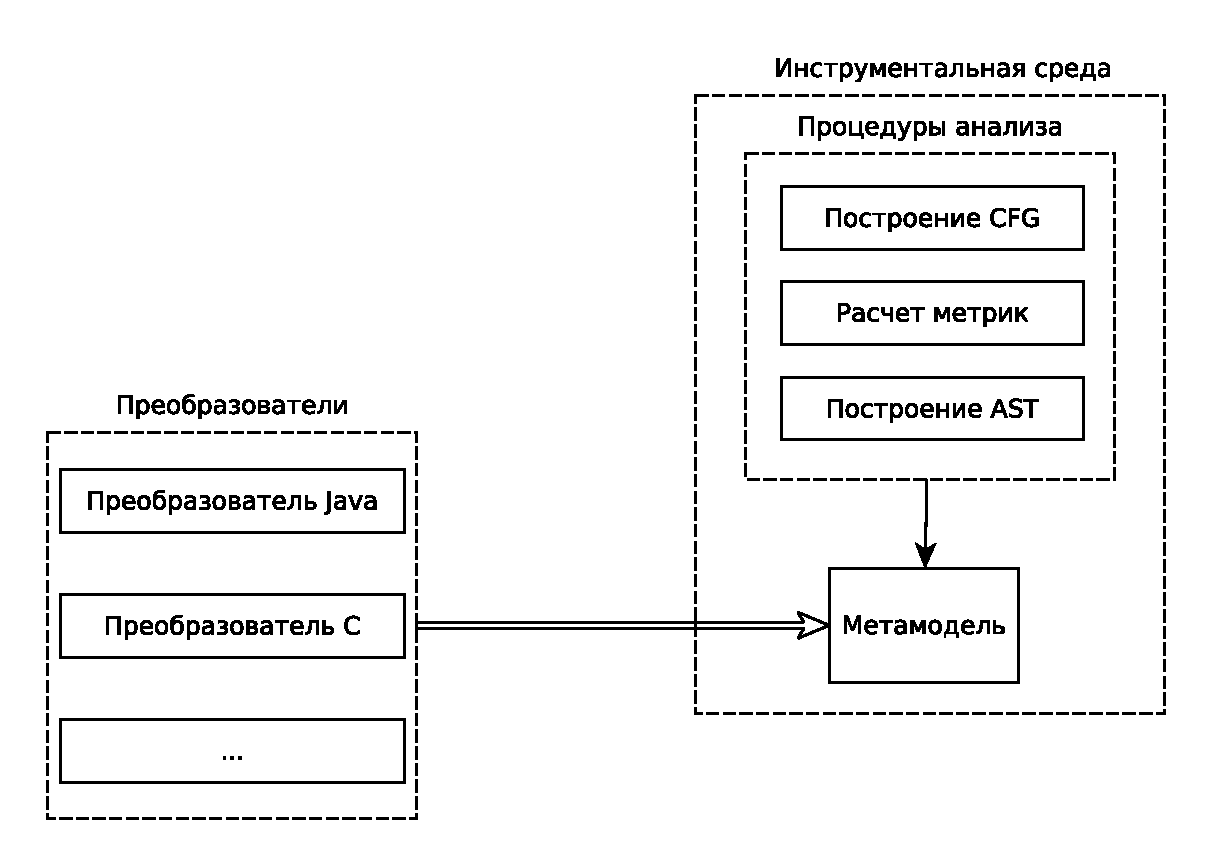
\includegraphics[width=0.9\textwidth]{fig/arch.eps}
    \end{center}
\end{figure}

\end{frame}
%===============================================================================
%===============================================================================
\begin{frame}
\frametitle{Принцип работы}

\begin{figure}[b!]
    \begin{center}
        \includegraphics<1 | handout:1>[width=0.9\textwidth]{fig/architecture.eps}
        \includegraphics<2 | handout:2>[width=0.9\textwidth]{fig/architecture2.eps}
        \includegraphics<3 | handout:3>[width=0.9\textwidth]{fig/architecture3.eps}
        \includegraphics<4 | handout:4>[width=0.9\textwidth]{fig/architecture4.eps}
        \includegraphics<5 | handout:5>[width=0.9\textwidth]{fig/architecture5.eps}
        \includegraphics<6 | handout:6>[width=0.9\textwidth]{fig/architecture6.eps}
        \includegraphics<7 | handout:7>[width=0.9\textwidth]{fig/architecture7.eps}
    \end{center}
\end{figure}

\end{frame}
%===============================================================================
%===============================================================================
\begin{frame}
\frametitle{Разработка метамодели}

\begin{itemize}
    \item Стандарт MOF - мета-метамодель
    \item Архитектура была модифицирована - убраны классы для отношений между
    сущностями
    \item Расширяемость - все сущности наследуются от одного класса
    \item API для обхода модели программы - шаблон ``Посетитель'' (Visitor)
\end{itemize}

\end{frame}
%===============================================================================
%===============================================================================
\begin{frame}
\frametitle{Разработка преобразователей}

\begin{itemize}
    \item Разрабатываются отдельно для каждого языка программирования
    \item Разработаны преобразователи для языков Java и C
    \item Для создания лексических и синтаксических анализаторов использовался
    генератор парсеров ANTLR
\end{itemize}

\end{frame}
%===============================================================================
%===============================================================================
\begin{frame}
\frametitle{Разработка процедур визуализации и анализа}

\begin{itemize}
    \item Графический интерфейс на Swing
    \item Для отрисовки графов используется библиотека JGraphX
    \item Визуализация AST и CFG
    \item Построение UML-диаграмм классов
        \begin{itemize}
            \item Существуют ограничения в силу недостаточного количества
            информации о семантике отношений
        \end{itemize}
    \item Подсчет метрик Лоренца и Кидда
\end{itemize}

\end{frame}
%===============================================================================
%===============================================================================
\begin{frame}[fragile]
\frametitle{Демонстрация}

Рассмотрим пример:

\begin{lstlisting}
class Condition {
  public static void main(String[] args) {
    boolean learning = true;

    if (learning) {
      System.out.println("Java programmer");
    } else {
      System.out.println("What are you doing here?");
    }
  }
}
\end{lstlisting}

\end{frame}
%===============================================================================
%===============================================================================
\begin{frame}
\frametitle{Демонстрация. Визуализация CFG}

\begin{figure}[h]
    \begin{center}
        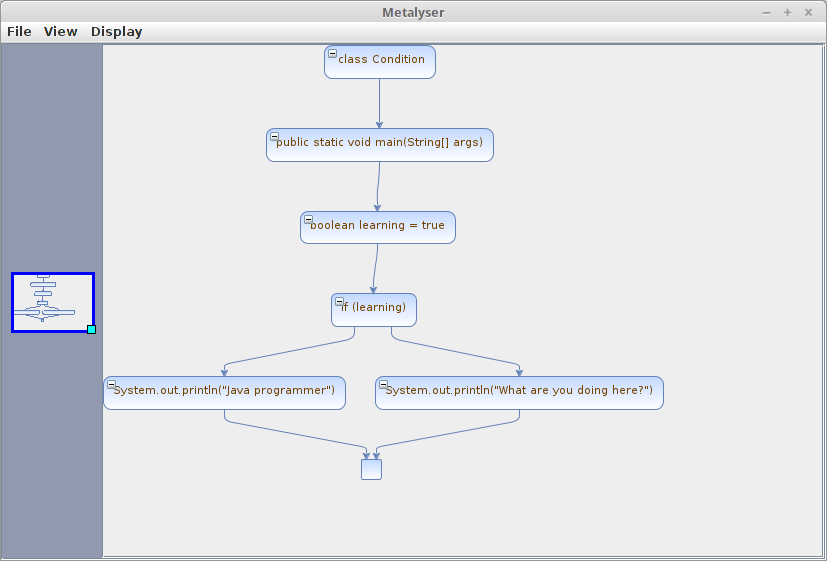
\includegraphics[width=0.9\textwidth]{../fig/cfg_test1.png}
    \end{center}
\end{figure}

\end{frame}
%===============================================================================
%===============================================================================
\begin{frame}
\frametitle{Демонстрация. Визуализация CFG}

\begin{figure}[b!]
    \begin{center}
        \includegraphics<1>[width=\textwidth]{fig/zoom1.png}
        \includegraphics<2>[width=\textwidth]{fig/zoom2.png}
        \includegraphics<3>[width=\textwidth]{fig/zoom3.png}
    \end{center}
\end{figure}

\end{frame}

%===============================================================================
%===============================================================================
\begin{frame}[fragile]
\frametitle{Демонстрация}
Еще один пример:

\begin{lstlisting}
public class umlTest {
    private final Test2 reference;
    private final Test3[] multipleReference;

    public void public1() {}

    public static void main(final String[] args) {}
}

class Test2 extends Super {
    private final int foo;
}

class Test3 extends Super {
    private final String bar;
}

class Super {
}
\end{lstlisting}

\end{frame}
%===============================================================================
%===============================================================================
\begin{frame}
\frametitle{Демонстрация. UML-диаграмма классов}

\begin{figure}[h]
    \begin{center}
        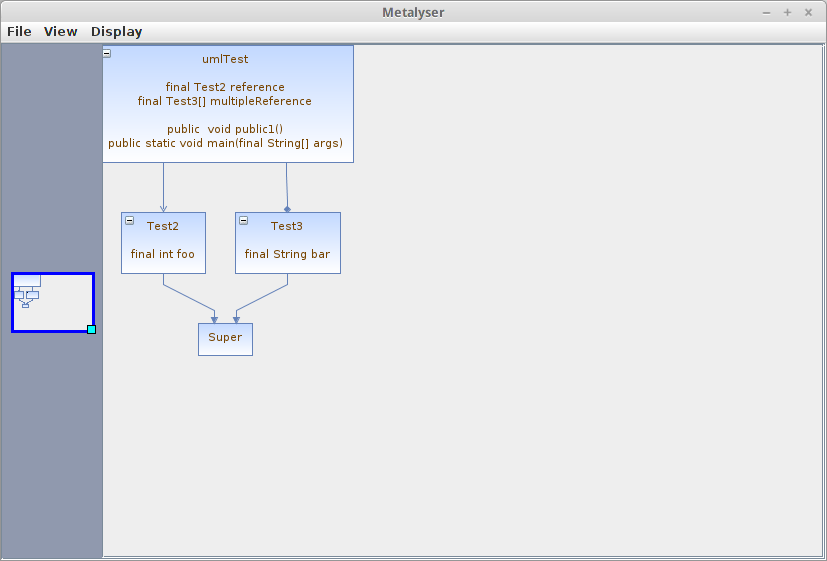
\includegraphics[width=0.9\textwidth]{fig/umlTest.png}
    \end{center}
\end{figure}

\end{frame}
%===============================================================================
%===============================================================================
\begin{frame}
\frametitle{Результаты}

\begin{itemize}
    \item Разработана языконезависимая метамодель для унификации процедур анализа
    и визуализации
    \item Разработана графическая инструментальная среда для демонстрации
    возможностей предложенного представления
    \item Проведено тестирование разработанной системы
    \item Разработанную метамодель можно применять в качестве библиотеки при
    создании анализаторов
\end{itemize}

\end{frame}
%===============================================================================
%===============================================================================
\begin{frame}
\frametitle{Направления дальнейшей разработки}

\begin{itemize}
    \item Разработка преобразователей для других языков программирования
    \item Извлечение новых видов моделей
    \item Создание языка запросов к метамодели
    \item Разработка новых видов визуализации
    \item Расчет дополнительных метрик
\end{itemize}

\end{frame}
%===============================================================================
%===============================================================================
\begin{frame}
\frametitle{Спасибо за внимание}
\center{\Huge{Спасибо за внимание!}}
\end{frame}
%===============================================================================

\end{document}
